\chapter*{Appendix E}\label{AppendixE}
\vspace{-1.75cm}
\subsection{Graphical posterior predictive checks}
%\label{subsection_model_checking}

Graphical posterior predictive checking is a valuable tool for visualizing the fit of the proposed model 
to the available data \shortcite{gelman_bayesian_2013}. The idea is straightforward: if the model is a good fit 
then it should be possible to simulate data from the model that resembles the observed data. Let $\Theta$ 
denote all parameters (including hyperparameters) in the hierarchical model. Following 
 \citeA{gelman_bayesian_2013}, $y^{\it rep}$ will be used to denote a {\it replication} of $y$ from the model.\footnote{\citeA{gelman_bayesian_2013} distinguishes between $y^{rep}$ and $\tilde{y}$. The former 
 makes use of the same explanatory variables/predictors $x$ used to estimate $\Theta$, while the latter 
 refers to predictions of future $y$ using potentially different variables $\tilde{x}$ (e.g. after collecting more data).}

For each draw of the parameters $\Theta$ from the posterior distribution $p(\Theta | y)$ an entire set 
of data $y^{\it rep} $ is simulated from the posterior predictive distribution

\begin{equation*}
 p(y^{\it rep} | y) = \int p(y^{\it rep}, \Theta | y) d\Theta = \int p(y^{\it rep} | \Theta) p(\Theta | y) d\Theta.
\end{equation*}

\noindent The posterior predictive distribution can thus be viewed as the likelihood for the new data 
$y^{\it rep}$ averaged over the posterior distribution  $p(\Theta | y)$.\footnote{
Intuitively, this corresponds to using the information about the parameters $\Theta$ learned from 
the observed $y$ to generate other plausible $y$'s.}

The histograms in Figure~\ref{fig:ck_pp_hists} (p. \pageref{fig:ck_pp_hists}) show the 
distribution of the observed data $y$ -- the number of roll-call votes won by the majority party 
-- alongside a selection replicated data sets $y^{\it rep}$ randomly chosen from all of the posterior 
predictive replications.\footnote{If $y$ is an $N$-vector and there are $D$ draws of 
$\Theta$ from $p(\Theta | y)$, then $D$ replicated data sets $y^{rep}$ will be simulated, 
each of which is also an $N$-vector. Figure~\ref{fig:ck_pp_hists} shows the distribution of $y$ and the
distributions of 15 of the replications.} This is a casual but informative comparison; it is an easy way 
of checking for inconsistencies due to poor model fit. In this case it shows that indeed the observed 
data are plausible under the posterior predictive distribution implied by the model. 


\begin{figure}[h]
\centering
	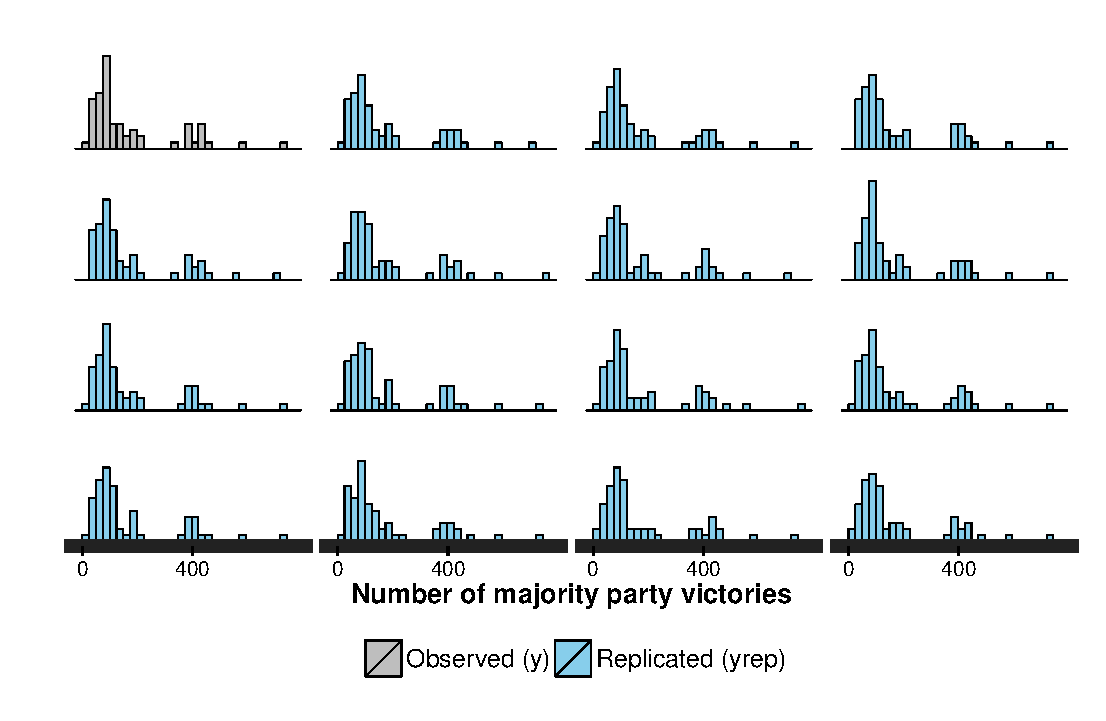
\includegraphics[scale=0.7]{sections/figs/ck_pp_y_vs_yrep_new}
\caption{Replications from posterior predictive distribution vs. observed data}
\label{fig:ck_pp_hists}
\end{figure}


Figure~\ref{fig:ck_pp_test_statistics} (p. \pageref{fig:ck_pp_test_statistics}) shows the distributions 
of the mean and standard deviation over all replications. The test statistics, denoted $T(y^{\it rep})$, 
are compared the observed values $T(y)$ computed from the data. 
In this case the observed values are nicely centered in the distributions of $T(y^{\it rep})$. 

\begin{figure}[h]
\centering
	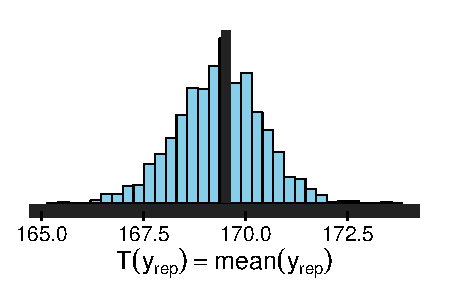
\includegraphics[scale=0.7]{sections/figs/test_stats_mean}
	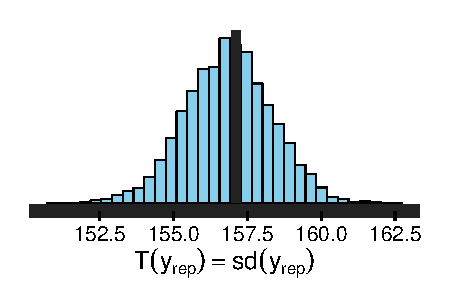
\includegraphics[scale=0.7]{sections/figs/test_stats_sd}
\caption{Distributions of test statistics $T(y_{rep})$. The vertical bar is the observed value $T(y)$.}
\label{fig:ck_pp_test_statistics}
\end{figure}


We should also look at the posterior predictive replications at the level of individual Congresses,
as this is the natural grouping in the data.  
Figure~\ref{fig:ck_pp_nWins_hists} (p. \pageref{fig:ck_pp_nWins_hists}) shows 
the distribution of $y^{\it rep}$ for each of the Congresses (i.e., time periods) in the data. 
Again, it is evident that the observations are consistent with the posterior predictive distribution.
% Should probably do pp checks after aggregating over the sub periods for each congress.  

\vspace{1cm}
\begin{figure}[h]
\centering
	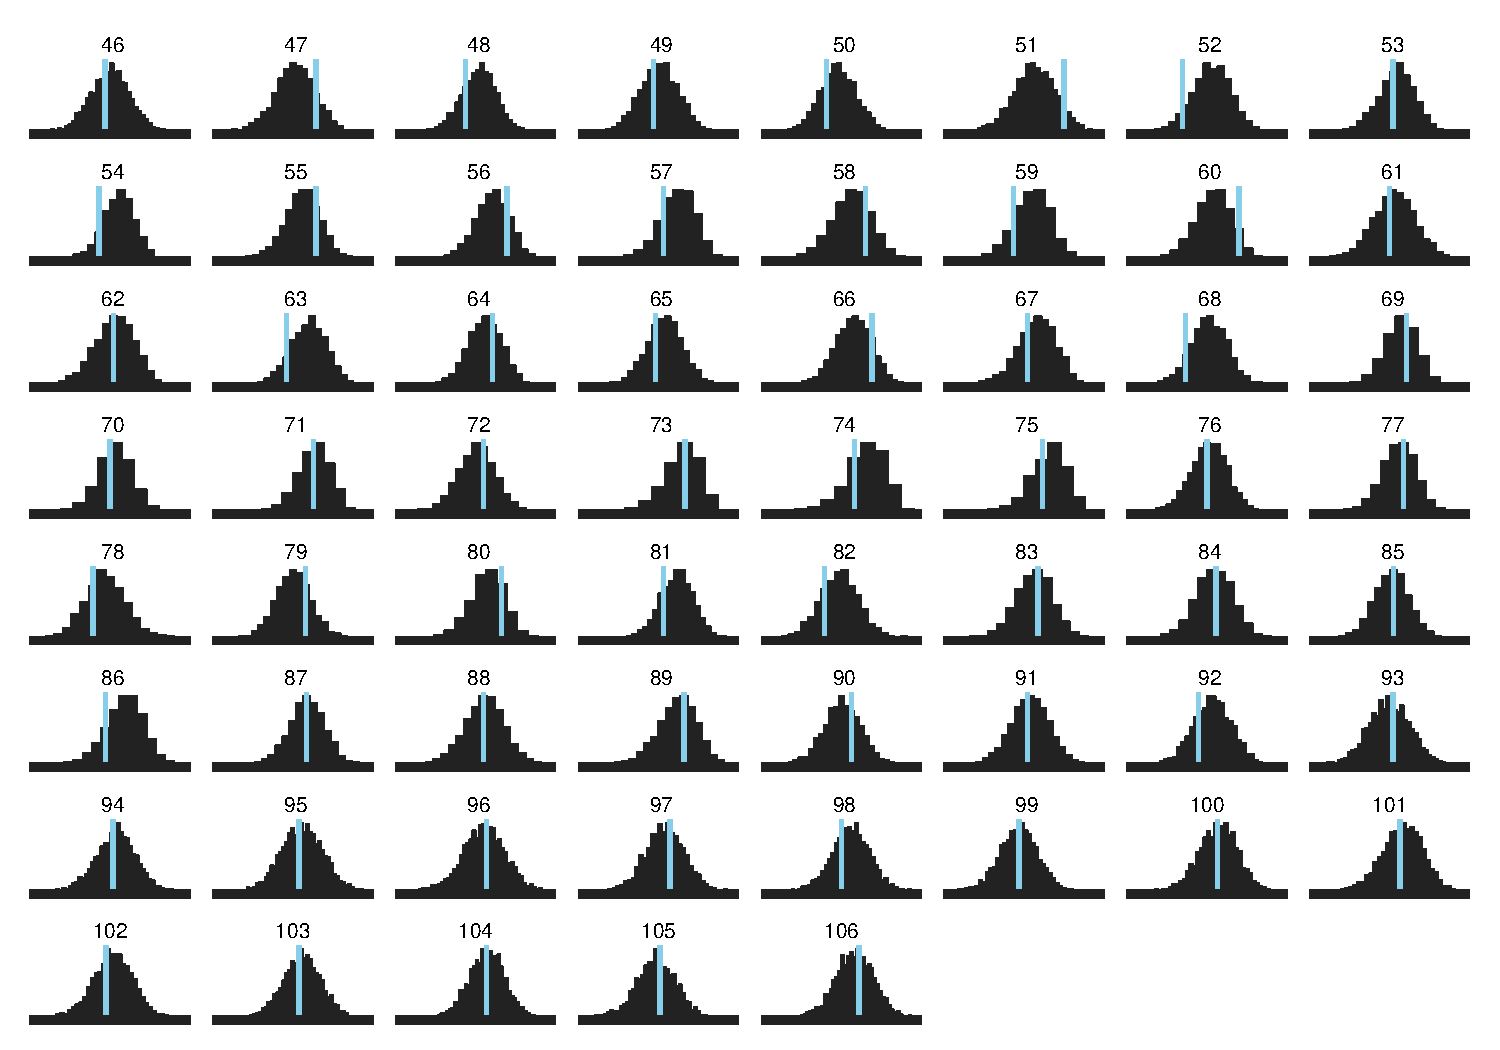
\includegraphics[scale=0.55]{sections/figs/ck_pp_by_cong}
\caption{Distributions of $y^{\it rep}$ by Congress. Vertical lines show observed values from the data.}
\label{fig:ck_pp_nWins_hists}
\end{figure}





